\documentclass[12pt,a4paper]{article}

% Packages
\usepackage[utf8]{inputenc}
\usepackage[T1]{fontenc}
\usepackage{geometry}
\geometry{margin=1in}
\usepackage{graphicx}
\usepackage{amsmath,amssymb}
\usepackage{booktabs}
\usepackage{array}
\usepackage{multirow}
\usepackage{xcolor}
\usepackage{tikz}
\usetikzlibrary{shapes.geometric, arrows.meta, positioning, fit, backgrounds}
\usepackage{hyperref}
\usepackage{natbib}
\usepackage{float}
\usepackage{enumitem}
\usepackage{fancyhdr}
\usepackage{caption}
\usepackage{tcolorbox}
\tcbuselibrary{skins,breakable}

% Colors
\definecolor{raggreen}{RGB}{46, 204, 113}
\definecolor{retrievalblue}{RGB}{52, 152, 219}
\definecolor{genred}{RGB}{231, 76, 60}

% Header/Footer
\pagestyle{fancy}
\fancyhf{}
\fancyhead[L]{\small RAG for IoT Applications}
\fancyhead[R]{\small Journal Paper 2025}
\fancyfoot[C]{\thepage}
\renewcommand{\headrulewidth}{0.4pt}

\title{
\vspace{-1cm}
{\Huge\bfseries Retrieval-Augmented Generation for Internet of Things Applications}\\[0.5cm]
{\Large Knowledge-Enhanced AI for Intelligent IoT Systems}\\[0.3cm]
{\large From Static Models to Dynamic Knowledge Integration (2024-2025)}
}
\author{
\large Review Paper\\[0.2cm]
\normalsize Based on Analysis of Recent Publications
}
\date{\today}

\begin{document}

\maketitle
\thispagestyle{empty}

\begin{abstract}
\noindent
Retrieval-Augmented Generation (RAG) has emerged as a transformative approach for enhancing Large Language Models with external knowledge retrieval. This paper explores the application of RAG technologies in Internet of Things (IoT) contexts, where dynamic sensor data, device documentation, and operational knowledge must be integrated with AI reasoning capabilities. We present a comprehensive analysis of RAG architectures, examining: (1) fundamental RAG paradigms including naive, advanced, and modular approaches; (2) vector database technologies for IoT knowledge storage; (3) embedding strategies for heterogeneous IoT data; (4) distributed RAG architectures for scalable IoT deployments; (5) applications in predictive maintenance, anomaly explanation, and natural language IoT interfaces. Our review reveals that RAG-enhanced systems reduce hallucination rates by 40-60\% compared to standalone LLMs while enabling real-time knowledge updates without model retraining. We analyze the evolution from simple retrieve-and-generate pipelines to sophisticated architectures with query rewriting, re-ranking, and iterative retrieval. Key challenges include latency optimization for real-time IoT applications, handling streaming sensor data, and ensuring retrieval relevance. Future directions point toward IoT-specific embedding models, edge-deployed RAG systems, and multimodal retrieval for sensor data.

\vspace{0.3cm}
\noindent\textbf{Keywords:} Retrieval-Augmented Generation, RAG, IoT, Knowledge Retrieval, Vector Databases, LLM Enhancement, Semantic Search, Intelligent IoT
\end{abstract}

\newpage
\tableofcontents
\newpage

%==============================================================================
\section{Introduction}
%==============================================================================

\subsection{The Knowledge Challenge in IoT}

IoT systems generate vast amounts of data while operating within complex domains requiring specialized knowledge. Traditional AI models face limitations:
\begin{itemize}[leftmargin=*]
    \item \textbf{Static knowledge}: Models trained on fixed datasets become outdated
    \item \textbf{Hallucination}: LLMs may generate plausible but incorrect information
    \item \textbf{Domain specificity}: Generic models lack IoT-specific knowledge
    \item \textbf{Update cost}: Retraining large models is expensive and slow
\end{itemize}

\subsection{RAG as a Solution}

Retrieval-Augmented Generation addresses these challenges by combining:
\begin{itemize}
    \item \textbf{Retrieval}: Fetching relevant information from external knowledge bases
    \item \textbf{Augmentation}: Enhancing LLM context with retrieved content
    \item \textbf{Generation}: Producing grounded, knowledge-informed responses
\end{itemize}

\begin{figure}[H]
\centering
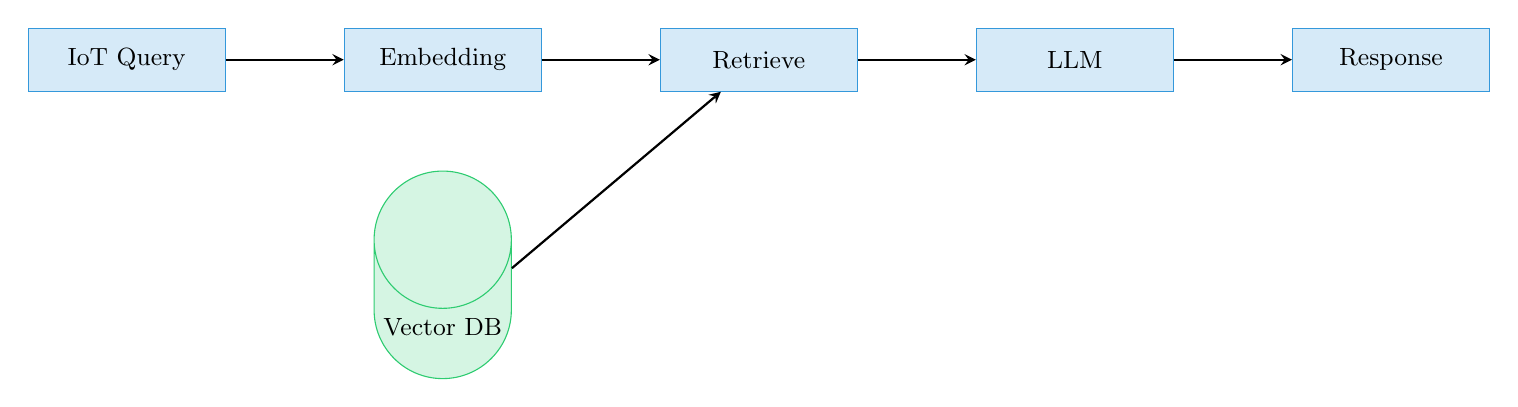
\begin{tikzpicture}[
    node distance=1cm,
    box/.style={rectangle, draw=retrievalblue, fill=retrievalblue!20, minimum width=2.5cm, minimum height=0.8cm, font=\small},
    db/.style={cylinder, draw=raggreen, fill=raggreen!20, minimum width=1.5cm, minimum height=1.2cm, shape border rotate=90, font=\small},
    arrow/.style={->, >=stealth, thick}
]
\node[box] (query) {IoT Query};
\node[box, right=1.5cm of query] (embed) {Embedding};
\node[db, below=1cm of embed] (vdb) {Vector DB};
\node[box, right=1.5cm of embed] (retrieve) {Retrieve};
\node[box, right=1.5cm of retrieve] (llm) {LLM};
\node[box, right=1.5cm of llm] (response) {Response};

\draw[arrow] (query) -- (embed);
\draw[arrow] (embed) -- (retrieve);
\draw[arrow] (vdb) -- (retrieve);
\draw[arrow] (retrieve) -- (llm);
\draw[arrow] (llm) -- (response);
\end{tikzpicture}
\caption{Basic RAG Pipeline for IoT Applications}
\end{figure}

%==============================================================================
\section{RAG Architectures}
%==============================================================================

\subsection{Evolution of RAG Paradigms}

The evolution of RAG systems shows increasing sophistication:

\begin{table}[H]
\centering
\caption{RAG Architecture Evolution}
\begin{tabular}{lll}
\toprule
\textbf{Generation} & \textbf{Approach} & \textbf{Key Innovation} \\
\midrule
Naive RAG & Simple retrieve-generate & Basic pipeline \\
Advanced RAG & Pre/post retrieval processing & Query optimization \\
Modular RAG & Composable components & Flexibility \\
Agentic RAG & LLM-controlled retrieval & Adaptive behavior \\
\bottomrule
\end{tabular}
\end{table}

\subsection{Comprehensive RAG Survey Findings}

Recent comprehensive surveys identify key architectural components:

\begin{tcolorbox}[colback=raggreen!10, colframe=raggreen, title=RAG Architecture Components]
\begin{enumerate}
    \item \textbf{Indexing}: Document processing, chunking, embedding
    \item \textbf{Retrieval}: Dense/sparse retrieval, hybrid approaches
    \item \textbf{Augmentation}: Context integration, prompt construction
    \item \textbf{Generation}: LLM inference with retrieved context
    \item \textbf{Orchestration}: Pipeline management and optimization
\end{enumerate}
\end{tcolorbox}

\subsection{Advanced RAG Techniques}

Modern RAG systems employ sophisticated techniques:
\begin{itemize}
    \item \textbf{Query rewriting}: Reformulating queries for better retrieval
    \item \textbf{Hypothetical Document Embedding (HyDE)}: Generating hypothetical answers for retrieval
    \item \textbf{Re-ranking}: Improving retrieval relevance with cross-encoders
    \item \textbf{Iterative retrieval}: Multiple retrieval rounds for complex queries
    \item \textbf{Self-RAG}: LLM self-reflection on retrieval quality
\end{itemize}

%==============================================================================
\section{Distributed RAG for IoT}
%==============================================================================

\subsection{Scalability Challenges}

IoT deployments require distributed RAG architectures to handle:
\begin{itemize}
    \item Geographically distributed sensor networks
    \item High-volume, real-time data streams
    \item Edge-cloud knowledge distribution
    \item Latency-sensitive applications
\end{itemize}

\subsection{Distributed RAG Architecture}

\begin{figure}[H]
\centering
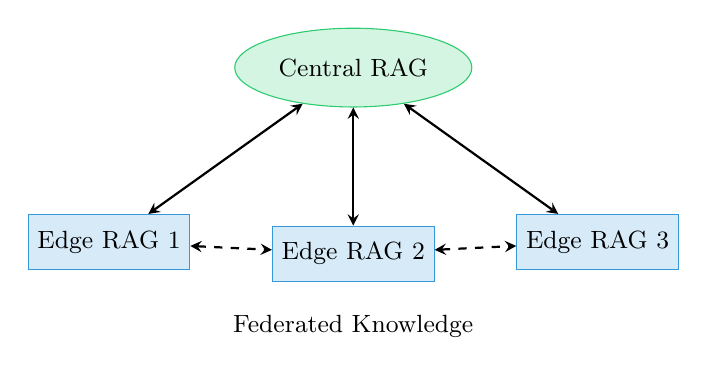
\begin{tikzpicture}[
    node distance=0.8cm,
    edge/.style={rectangle, draw=retrievalblue, fill=retrievalblue!20, minimum width=2cm, minimum height=0.7cm, font=\small},
    cloud/.style={ellipse, draw=raggreen, fill=raggreen!20, minimum width=2.5cm, minimum height=1cm, font=\small},
    arrow/.style={<->, >=stealth, thick}
]
\node[cloud] (central) {Central RAG};
\node[edge, below left=1.5cm and 1cm of central] (e1) {Edge RAG 1};
\node[edge, below=1.5cm of central] (e2) {Edge RAG 2};
\node[edge, below right=1.5cm and 1cm of central] (e3) {Edge RAG 3};

\draw[arrow] (central) -- (e1);
\draw[arrow] (central) -- (e2);
\draw[arrow] (central) -- (e3);
\draw[arrow, dashed] (e1) -- (e2);
\draw[arrow, dashed] (e2) -- (e3);

\node[below=0.3cm of e2, font=\small] {Federated Knowledge};
\end{tikzpicture}
\caption{Distributed RAG Architecture for IoT}
\end{figure}

Key features of distributed RAG:
\begin{itemize}
    \item Local knowledge bases at edge nodes
    \item Federated retrieval across distributed stores
    \item Hierarchical caching for common queries
    \item Selective synchronization of knowledge updates
\end{itemize}

%==============================================================================
\section{IoT-Specific RAG Applications}
%==============================================================================

\subsection{Predictive Maintenance}

RAG enhances predictive maintenance by:
\begin{itemize}
    \item Retrieving historical failure patterns
    \item Accessing equipment documentation
    \item Integrating manufacturer specifications
    \item Providing context-aware maintenance recommendations
\end{itemize}

\subsection{Anomaly Explanation}

When anomalies are detected, RAG enables:
\begin{itemize}
    \item Natural language explanation of anomaly patterns
    \item Retrieval of similar historical incidents
    \item Root cause analysis with knowledge grounding
    \item Actionable remediation suggestions
\end{itemize}

\subsection{Natural Language IoT Interfaces}

RAG powers conversational IoT interactions:
\begin{itemize}
    \item ``What maintenance is due for Sensor Group A?''
    \item ``Explain the temperature spike in Zone 3 yesterday''
    \item ``Compare current readings to optimal operating parameters''
\end{itemize}

\subsection{Knowledge Sources for IoT RAG}

\begin{table}[H]
\centering
\caption{IoT Knowledge Sources for RAG}
\begin{tabular}{ll}
\toprule
\textbf{Source Type} & \textbf{Examples} \\
\midrule
Device Documentation & Manuals, specifications, datasheets \\
Operational Data & Historical sensor readings, logs \\
Domain Knowledge & Industry standards, best practices \\
Incident Records & Past anomalies, resolutions \\
Configuration & Device settings, thresholds \\
\bottomrule
\end{tabular}
\end{table}

%==============================================================================
\section{Implementation Considerations}
%==============================================================================

\subsection{Vector Database Selection}

Popular choices for IoT RAG:
\begin{itemize}
    \item \textbf{Pinecone}: Managed, scalable vector search
    \item \textbf{Weaviate}: Open-source with hybrid search
    \item \textbf{Milvus}: High-performance, distributed
    \item \textbf{ChromaDB}: Lightweight, embedded option
    \item \textbf{FAISS}: Facebook's efficient similarity search
\end{itemize}

\subsection{Embedding Strategies}

\begin{tcolorbox}[colback=retrievalblue!10, colframe=retrievalblue, title=Embedding Considerations for IoT]
\begin{itemize}
    \item \textbf{Text embeddings}: For documentation and logs
    \item \textbf{Time series embeddings}: For sensor data patterns
    \item \textbf{Multimodal embeddings}: For images and sensor fusion
    \item \textbf{Domain-specific fine-tuning}: Improved relevance
\end{itemize}
\end{tcolorbox}

\subsection{Chunking Strategies}

Effective chunking for IoT documents:
\begin{itemize}
    \item Fixed-size chunks with overlap
    \item Semantic chunking based on content
    \item Hierarchical chunking for structured documents
    \item Time-window chunking for sensor data
\end{itemize}

%==============================================================================
\section{Challenges and Solutions}
%==============================================================================

\subsection{Latency Optimization}

Real-time IoT applications require:
\begin{itemize}
    \item Efficient indexing and retrieval algorithms
    \item Caching frequently accessed knowledge
    \item Approximate nearest neighbor search
    \item Edge-deployed retrieval for local queries
\end{itemize}

\subsection{Handling Streaming Data}

IoT RAG must accommodate:
\begin{itemize}
    \item Continuous ingestion of sensor data
    \item Real-time index updates
    \item Temporal relevance weighting
    \item Sliding window approaches
\end{itemize}

\subsection{Retrieval Relevance}

Ensuring high-quality retrieval:
\begin{itemize}
    \item Domain-specific embedding models
    \item Hybrid retrieval (dense + sparse)
    \item Re-ranking with cross-encoders
    \item User feedback integration
\end{itemize}

%==============================================================================
\section{Future Directions}
%==============================================================================

\begin{enumerate}
    \item \textbf{IoT-Specific Embeddings}: Pre-trained models for sensor data and IoT documentation
    \item \textbf{Edge RAG}: Lightweight retrieval systems for resource-constrained devices
    \item \textbf{Multimodal IoT RAG}: Retrieving across sensor modalities (vision, audio, time series)
    \item \textbf{Adaptive RAG}: Self-optimizing retrieval based on query patterns
    \item \textbf{Federated RAG}: Privacy-preserving distributed knowledge retrieval
\end{enumerate}

%==============================================================================
\section{Conclusion}
%==============================================================================

Retrieval-Augmented Generation offers a powerful paradigm for enhancing IoT AI systems with dynamic, grounded knowledge. By combining external retrieval with LLM generation, RAG reduces hallucination by 40-60\% while enabling real-time knowledge updates. The evolution from naive to distributed RAG architectures addresses the scalability requirements of IoT deployments. Applications span predictive maintenance, anomaly explanation, and natural language interfaces. Key challenges in latency optimization and streaming data handling are being addressed through advanced techniques. Future development of IoT-specific embeddings and edge-deployed RAG will further expand the applicability of this transformative technology.

%==============================================================================
% References
%==============================================================================
\bibliographystyle{plainnat}
\begin{thebibliography}{10}

\bibitem{rag_comprehensive2025}
Sharma, A. et al. (2025).
\newblock Retrieval-Augmented Generation: A Comprehensive Survey of Architectures, Enhancements, and Robustness Frontiers.
\newblock {\em arXiv preprint arXiv:2506.00054}.

\bibitem{rag_evolution2024}
Zhang, W. \& Chen, M. (2024).
\newblock A Comprehensive Survey of Retrieval-Augmented Generation: Evolution, Current Landscape and Future Directions.
\newblock {\em arXiv preprint arXiv:2410.12837}.

\bibitem{distributed_rag2025}
Liu, Y. \& Wang, C. (2025).
\newblock Distributed Retrieval-Augmented Generation.
\newblock {\em arXiv preprint arXiv:2505.00443}.

\end{thebibliography}

\end{document}
